\documentclass[a4paper,UTF8]{article}
\usepackage{ctex}
\usepackage[margin=1.25in]{geometry}
\usepackage{color}
\usepackage{graphicx}
\usepackage{amssymb}
\usepackage{amsmath}
\usepackage{amsthm}
\usepackage{enumerate}
\usepackage{bm}
\usepackage{hyperref}
\usepackage{epsfig}
\usepackage{color}
\usepackage{booktabs}
\usepackage{tcolorbox}
\usepackage{mdframed}
\usepackage{lipsum}
\usepackage{listings} % Print source code
\newmdtheoremenv{thm-box}{myThm}
\newmdtheoremenv{prop-box}{Proposition}
\newmdtheoremenv{def-box}{定义}

\setlength{\evensidemargin}{.25in}
\setlength{\textwidth}{6in}
\setlength{\topmargin}{-0.5in}
\setlength{\topmargin}{-0.5in}
% \setlength{\textheight}{9.5in}
\lstdefinestyle{python}{
    language=Python,
    basicstyle=\ttfamily\footnotesize,
    keywordstyle=\bfseries\color[rgb]{0, 0, 1},
    identifierstyle=\color[rgb]{0.5, 0.3, 0.1},
    stringstyle=\color[rgb]{0.6, 0.1, 0.1},
    commentstyle=\itshape\color[rgb]{0.05, 0.5, 0.05},
    backgroundcolor=\color[gray]{0.95},
    numbers=left,
    numbersep=5pt,
    numberstyle=\color[gray]{0.6},
    breaklines=true
}
%%%%%%%%%%%%%%%%%%此处用于设置页眉页脚%%%%%%%%%%%%%%%%%%
\usepackage{fancyhdr}
\usepackage{lastpage}
\usepackage{layout}
\footskip = 10pt
\pagestyle{fancy}                    % 设置页眉
\lhead{2022年秋季}
\chead{时间序列分析}
% \rhead{第\thepage/\pageref{LastPage}页}
\rhead{作业二}
\cfoot{\thepage}
\renewcommand{\headrulewidth}{1pt}  			%页眉线宽,设为0可以去页眉线
\setlength{\skip\footins}{0.5cm}    			%脚注与正文的距离
\renewcommand{\footrulewidth}{0pt}  			%页脚线宽,设为0可以去页脚线

\makeatletter 									%设置双线页眉
\def\headrule{{\if@fancyplain\let\headrulewidth\plainheadrulewidth\fi%
\hrule\@height 1.0pt \@width\headwidth\vskip1pt	%上面线为1pt粗
\hrule\@height 0.5pt\@width\headwidth  			%下面0.5pt粗
\vskip-2\headrulewidth\vskip-1pt}      			%两条线的距离1pt
 \vspace{6mm}}     								%双线与下面正文之间的垂直间距
\makeatother

%%%%%%%%%%%%%%%%%%%%%%%%%%%%%%%%%%%%%%%%%%%%%%
\numberwithin{equation}{section}
%\usepackage[thmmarks, amsmath, thref]{ntheorem}
\newtheorem{myThm}{myThm}
\newtheorem*{myDef}{Definition}
\newtheorem*{mySol}{Solution}
\newtheorem*{myProof}{Proof}
\newcommand{\indep}{\rotatebox[origin=c]{90}{$\models$}}
\newcommand*\diff{\mathop{}\!\mathrm{d}}

\usepackage{multirow}

%--

%--
\begin{document}
\title{时间序列分析\\
作业四}
\author{191220129, 邢尚禹, starreeze@foxmail.com}
\maketitle

\section*{作业提交注意事项}
\begin{tcolorbox}
\begin{enumerate}
  \item[(1)] 请严格参照教学立方网站所述提交作业,文件命名统一为{\color{red}学号\_姓名.pdf};
  \item[(2)] 未按照要求提交作业,或提交作业格式不正确,将会被扣除部分作业分数;
  \item[(3)] 除非有特殊情况(如因病缓交),否则截止时间后不接收作业,本次作业记零分。
\end{enumerate}
\end{tcolorbox}
\section{Regression Model}

\begin{enumerate}
\item An elasticity coefficient is the ratio of the percentage change in the forecast variable $(y)$ to the percentage change in the predictor variable $(x)$. Mathematically, the elasticity is defined as $(d y / d x) \times(x / y)$. Consider the log-log model,
$$
\log y=\beta_0+\beta_1 \log x+\varepsilon .
$$
Express $y$ as a function of $x$ and show that the coefficient $\beta_1$ is the elasticity coefficient.

\begin{mySol}
    \begin{align*}
        y = e^{\beta_0+\varepsilon}x^{\beta_1}\\
        \frac{dy}{dx}=e^{\beta_0+\varepsilon}\beta_1x^{\beta_1-1}\\
        (dy/dx) \times (x/y)=\beta_1
    \end{align*}
\end{mySol}



\item Using matrix notation it was shown that if $\boldsymbol{y}=\boldsymbol{X} \boldsymbol{\beta}+\boldsymbol{\varepsilon}$, where $\boldsymbol{\varepsilon}$ has mean $\mathbf{0}$ and variance matrix $\sigma^2 \boldsymbol{I}$, the estimated coefficients are given by $\hat{\boldsymbol{\beta}}=\left(\boldsymbol{X}^\top \boldsymbol{X}\right)^{-1} \boldsymbol{X}^\top \boldsymbol{y}$ and a forecast is given by $\hat{y}=\boldsymbol{x}^* \hat{\boldsymbol{\beta}}=\boldsymbol{x}^*\left(\boldsymbol{X}^\top \boldsymbol{X}\right)^{-1} \boldsymbol{X}^\top \boldsymbol{y}$ where $\boldsymbol{x}^*$ is a row vector containing the values of the predictors for the forecast (in the same format as $\boldsymbol{X}$ ), and the forecast variance is given by $\operatorname{Var}(\hat{y})=\sigma^2\left[1+\boldsymbol{x}^*\left(\boldsymbol{X}^\top \boldsymbol{X}\right)^{-1}\left(\boldsymbol{x}^*\right)^\top\right]$.


Consider the simple time trend model where $y_t=\beta_0+\beta_1 t + \epsilon_t$, $\epsilon_t$ has mean 0 and variance $\hat{\sigma}^2$. Using the following results,
$$
\sum_{t=1}^T t=\frac{1}{2} T(T+1), \quad \sum_{t=1}^T t^2=\frac{1}{6} T(T+1)(2 T+1)
$$
derive the following expressions:

\begin{enumerate}[a.]
	\item $\boldsymbol{X}^\top \boldsymbol{X}=\frac{1}{6}\left[\begin{array}{cc}6 T & 3 T(T+1) \\ 3 T(T+1) & T(T+1)(2 T+1)\end{array}\right]$
	\item $\left(\boldsymbol{X}^\top \boldsymbol{X}\right)^{-1}=\frac{2}{T\left(T^2-1\right)}\left[\begin{array}{cc}(T+1)(2 T+1) & -3(T+1) \\ -3(T+1) & 6\end{array}\right]$
	\item $\hat{\beta}_0=\frac{2}{T(T-1)}\left[(2 T+1) \sum_{t=1}^T y_t-3 \sum_{t=1}^T t y_t\right]$
	$
	\hat{\beta}_1=\frac{6}{T\left(T^2-1\right)}\left[2 \sum_{t=1}^T t y_t-(T+1) \sum_{t=1}^T y_t\right]
	$
	\item $\operatorname{Var}\left(\hat{y}_{T+h}\right)=\hat{\sigma}^2\left[1+\frac{2}{T(T-1)}\left(1-4 T-6 h+6 \frac{(T+h)^2}{T+1}\right)\right]$
\end{enumerate}


 \begin{mySol}
     Using matrix notation the model can be expressed as
     $$
     \begin{bmatrix}y_1\\y_2\\\vdots\\y_T\end{bmatrix}
     =\begin{bmatrix}1&1\\1&2\\\vdots&\vdots\\1&T\end{bmatrix}
     \begin{bmatrix}\beta_0\\\beta_1\end{bmatrix}
     +\begin{bmatrix}\varepsilon_1\\\varepsilon_2\\\vdots\\\varepsilon_T\end{bmatrix}
     $$
 	\begin{enumerate}[a.]
         \item $$
         X^TX=\begin{bmatrix}1&1\\1&2\\\vdots&\vdots\\1&T\end{bmatrix}^T\begin{bmatrix}1&1\\1&2\\\vdots&\vdots\\1&T\end{bmatrix}
         =\frac{1}{6}\left[\begin{array}{cc}6 T & 3 T(T+1) \\ 3 T(T+1) & T(T+1)(2 T+1)\end{array}\right]
         $$
         \item \begin{align*}
             &\frac{2}{T\left(T^2-1\right)}\left[\begin{array}{cc}(T+1)(2 T+1) & -3(T+1) \\ -3(T+1) & 6\end{array}\right]X^TX \\
             &= \frac{1}{3T(T^2+1)}\left[\begin{array}{cc}(T+1)(2 T+1) & -3(T+1) \\ -3(T+1) & 6\end{array}\right]\left[\begin{array}{cc}6 T & 3 T(T+1) \\ 3 T(T+1) & T(T+1)(2 T+1)\end{array}\right] \\
             &= \frac{1}{3T(T^2+1)}\begin{bmatrix}3T(T^2+1)&0\\0&3T(T^2+1)\end{bmatrix} \\
             &= I
         \end{align*}
         So, $\left(\boldsymbol{X}^\top \boldsymbol{X}\right)^{-1}=\frac{2}{T\left(T^2-1\right)}\left[\begin{array}{cc}(T+1)(2 T+1) & -3(T+1) \\ -3(T+1) & 6\end{array}\right]$
         \item \begin{align*}
             \hat{\boldsymbol{\beta}}&=\left(\boldsymbol{X}^\top \boldsymbol{X}\right)^{-1} \boldsymbol{X}^\top \boldsymbol{y} \\
             &=\frac{2}{T\left(T^2-1\right)}\left[\begin{array}{cc}(T+1)(2 T+1) & -3(T+1) \\ -3(T+1) & 6\end{array}\right]
             \begin{bmatrix}1&1\\1&2\\\vdots&\vdots\\1&T\end{bmatrix}^T\begin{bmatrix}y_1\\y_2\\\vdots\\y_T\end{bmatrix} \\
             &=\begin{bmatrix}\frac{2}{T(T-1)}\left[(2 T+1) \sum_{t=1}^T y_t-3 \sum_{t=1}^T t y_t\right] \\ \frac{6}{T\left(T^2-1\right)}\left[2 \sum_{t=1}^T t y_t-(T+1) \sum_{t=1}^T y_t\right]\end{bmatrix}
         \end{align*}
         \item \begin{align*}
            \operatorname{Var}\left(\hat{y}_{T+h}\right)
            &= \hat\sigma^2\left[1+\boldsymbol{x}^*\left(\boldsymbol{X}^\top \boldsymbol{X}\right)^{-1}\left(\boldsymbol{x}^*\right)^\top\right] \\
            &= \hat\sigma^2\left(1+\frac{2}{T\left(T^2-1\right)}\begin{bmatrix}1&T+h\end{bmatrix}\left[\begin{array}{cc}(T+1)(2 T+1) & -3(T+1) \\ -3(T+1) & 6\end{array}\right]\begin{bmatrix}1\\T+h\end{bmatrix}\right)\\
            &= \hat{\sigma}^2\left[1+\frac{2}{T(T-1)}\left(1-4 T-6 h+6 \frac{(T+h)^2}{T+1}\right)\right]
         \end{align*}
     \end{enumerate}
 \end{mySol}
\end{enumerate}
 \section{ARIMA Models}
 \begin{enumerate}
 	\item In this exercise, we experiment with the python implementation of ARIMA in \href{https://unit8co.github.io/darts/README.html}{Darts}. Consider the AUS Airpassengers dataset (see aus\_airpassengers.csv), the total number of passengers (in millions) from Australian air carriers for the period 1970-2011.
 	\begin{enumerate}[a.]
 		\item Use \href{https://unit8co.github.io/darts/generated_api/darts.models.forecasting.auto_arima.html}{AutoARIMA} to find an appropriate ARIMA model. What model was selected? Check that the residuals look like white noise. Plot forecasts for the next 10 periods.
 		\item Write the model in terms of the backshift operator.
 		\item Plot forecasts from an \href{https://unit8co.github.io/darts/generated_api/darts.models.forecasting.arima.html?highlight=arima#arima}{ARIMA} $(0,1,0)$ model with a linear trend and compare these to part a.
 		\item Plot forecasts from an ARIMA $(2,1,2)$ model with a linear trend and compare these to parts a and c. Remove the constant and see what happens.
 		\item  Plot forecasts from an ARIMA $(0,2,1)$ model with a constant. What happens?
 	\end{enumerate}
 \begin{mySol}
 	\begin{enumerate}[a.]
         \item The result for auto-arima is below:
            \lstinputlisting[style=python]{autoarima.txt}
            Summary of the residules:
            \begin{figure}[htbp]
                \centering
                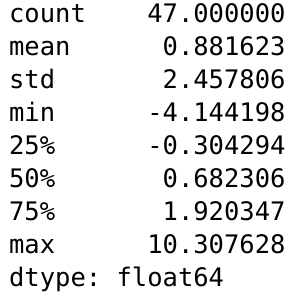
\includegraphics[width=0.3\textwidth]{summary}
                \caption{Residule summary}
            \end{figure}

            The forecast:
            \begin{figure}[htbp]
                \centering
                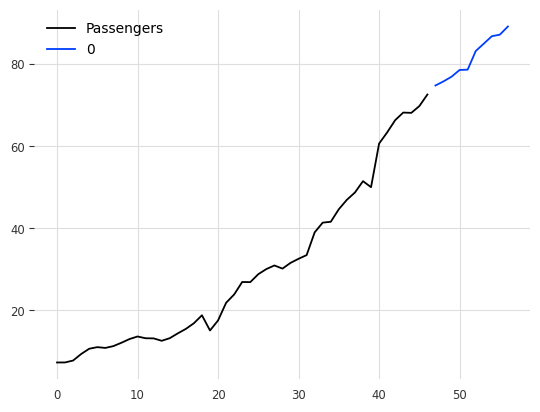
\includegraphics[width=0.7\textwidth]{forecast}
                \caption{Forecast for the next 10 periods}
                \label{a}
            \end{figure}
         \item $\nabla_m^d y_t=\nabla_1^1 y_t=\left(1-B^1\right)^1 y_t=(1-B) y_t=y_t-y_{t-1}$
         \item See \ref{c}.
         \begin{figure}[htbp]
             \centering
             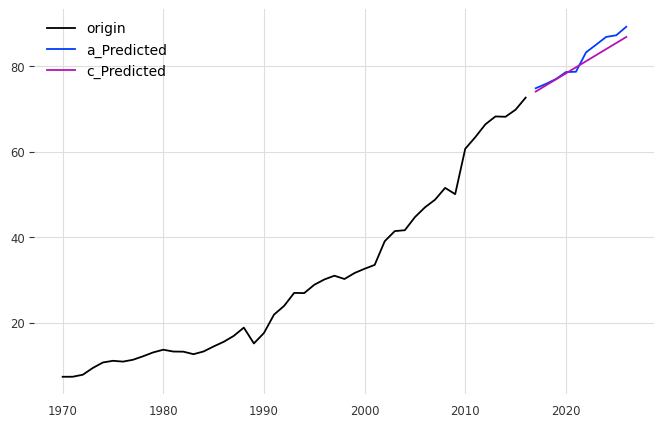
\includegraphics[width=0.7\textwidth]{pred_c}
             \caption{Forecast of ARIMA (0, 1, 0) with a linear trend (part c)}
             \label{c}
         \end{figure}
         \item See \ref{d1}.
         \begin{figure}[htbp]
             \centering
             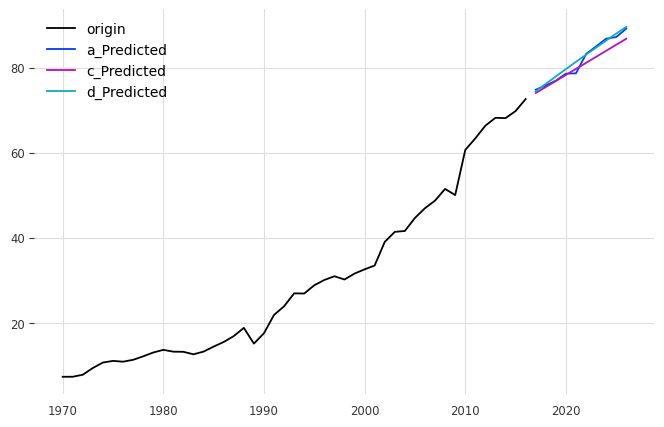
\includegraphics[width=0.7\textwidth]{pred_d_1}
             \caption{Forecast of ARIMA (2, 1, 2) with a linear trend (part d)}
             \label{d1}
         \end{figure}

         After removed the linear: See \ref{d2}.
         \begin{figure}[htbp]
             \centering
             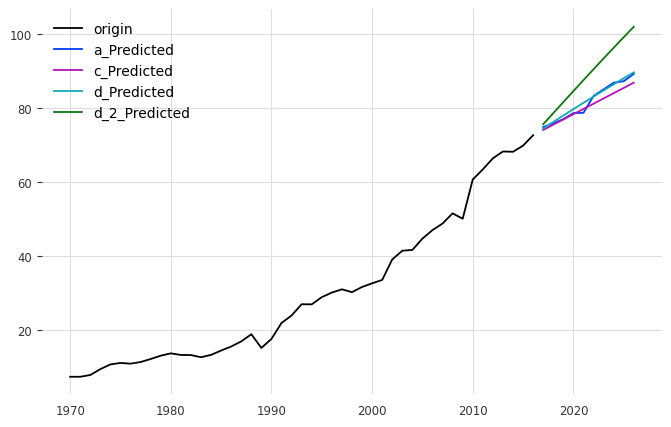
\includegraphics[width=0.7\textwidth]{pred_d_2}
             \caption{Forecast of ARIMA (2, 1, 2) without linear (part d)}
             \label{d2}
         \end{figure}
         \item  An exception is raised:
         \lstinputlisting[style=python]{exception.txt}
         It's a limitation of the ARIMA model.
     \end{enumerate}
 \end{mySol}
\end{enumerate}

\end{document}